\documentclass[11pt]{article}

% ============================================================================
%  РУССКАЯ версия статьи. Английский оригинал — main.tex; общие refs.bib и
%  fig_transfer.pdf. Собирать: pdflatex -> bibtex -> pdflatex x2.
%  \artifacturl задаётся в ОДНОМ месте (ниже), как и в английской версии.
% ============================================================================

\usepackage[utf8]{inputenc}
\usepackage[T2A]{fontenc}
\usepackage[english,russian]{babel}
\usepackage{lmodern}
\usepackage{amsmath,amssymb,amsthm}
\usepackage{booktabs}
\usepackage{graphicx}
\usepackage[expansion=false]{microtype}
\usepackage{xcolor}
\usepackage[margin=1in]{geometry}
\usepackage[numbers,sort&compress]{natbib}
\usepackage[unicode,colorlinks=true,linkcolor=blue!55!black,citecolor=blue!55!black,urlcolor=blue!55!black]{hyperref}
\usepackage{url}

\newtheorem{proposition}{Утверждение}

\newcommand{\inner}[2]{\langle #1,\, #2\rangle}
\newcommand{\fto}{\texorpdfstring{FHEW$\to$CKKS}{FHEW-to-CKKS}}
\newcommand{\ctf}{\texorpdfstring{CKKS$\to$FHEW}{CKKS-to-FHEW}}
\newcommand{\Z}{\mathbb{Z}}
\newcommand{\out}{\mathsf{out}}
\newcommand{\code}[1]{\texttt{#1}}
% TODO: задать \artifacturl адресом запушенного репозитория, затем пересобрать.
\newcommand{\artifacturl}{https://github.com/almantare/fhew-to-ckks-indcpad}

\title{\bfseries Восстановление секретного ключа FHEW из переключения схем\\ \fto{} в модели IND-CPA-D}

\author{%
  Артемий Алтамаре\\[2pt]
  \small НИУ ВШЭ, МИЭМ, Москва\\
  \small \texttt{aaaltamare@edu.hse.ru}%
}
\date{\today}

\begin{document}
\maketitle

\begin{abstract}
\citeauthor{santato2026}~\cite{santato2026} показывают, что преобразование шифротекста CKKS в
FHEW позволяет противнику в модели IND-CPA-D обойти контрмеру зашумления CKKS и восстановить
секретный ключ CKKS. Они реализуют атаку против OpenFHE, но проверяют только направление \ctf{},
явно отмечая, что OpenFHE переключает <<in both directions; we focus only on the
CKKS-to-FHEW direction>>. Мы закрываем второе направление. Преобразование \fto{} в OpenFHE
гомоморфно вычисляет расшифрование LWE; мы \emph{измеряем} его передаточную функцию:
$\out = (p/2\pi)\sin(2\pi\,\varphi/q)$, так что возвращаемое сообщение CKKS --- это сообщение LWE
\emph{плюс ошибка LWE, ослабленная масштабирующим множителем}. Переключение лишь уменьшает ошибку, и она попадает в пространство сообщений целевой схемы. Это делает
атаку немедленной в игре IND-CPA-D: запросить шифрование нуля, применить оракул переключения и
запросить расшифрование. Обращение синуса точно восстанавливает ошибку каждого шифротекста, что
даёт линейное уравнение относительно секрета LWE. Поскольку одно переключение упаковывает много
шифротекстов LWE в слоты CKKS, один запрос на расшифрование даёт $512$ уравнений, а
\textbf{три запроса восстанавливают весь $1305$-координатный секретный ключ FHEW STD128} (проверено
end-to-end, $1536/1536$ ошибок точно). Общее утверждение: переключение схем переносит ошибку
\emph{исходной} схемы в сообщение \emph{целевой}, поэтому оракул расшифрования на целевой схеме
восстанавливает секрет исходной. Это направление важно на практике, потому что все развёрнутые
контрмеры рассчитаны на ошибку CKKS, а ошибку LWE не защищает ничто, поскольку FHEW считают
точной схемой. Собственное зашумление OpenFHE, выкрученное
до максимума, который принимает библиотека, атаку \textbf{не} останавливает; зашумление,
откалиброванное по распространяемому шумовому тегу (Алгоритм~6 в~\cite{santato2026}), ---
останавливает.
\end{abstract}

\section{Введение}

Библиотеки полностью гомоморфного шифрования (FHE) всё чаще поддерживают \emph{переключение схем}:
преобразование шифротекста одной схемы FHE в шифротекст другой, чтобы каждая схема использовалась
там, где она сильнее всего --- CKKS~\cite{cheon2017} для SIMD-арифметики над вещественными числами,
FHEW/TFHE~\cite{ducas2015} для быстрых булевых вентилей и сравнений. OpenFHE~\cite{openfhe}
поставляет эту возможность для CKKS и FHEW в обоих направлениях.

CKKS --- \emph{приближённая} схема: расшифрование возвращает сообщение плюс малую ошибку.
\citeauthor{limicciancio2021}~\cite{limicciancio2021} показали, что из-за этого <<учебный>> CKKS
небезопасен в модели IND-CPA-D (неразличимость при атаке с выбранным открытым текстом и оракулом
расшифрования), поскольку возвращаемая ошибка --- линейная функция секретного ключа. Стандартная
контрмера --- \emph{зашумление} (noise flooding): перед возвратом расшифрованного значения к нему
добавляют случайный шум, достаточно большой, чтобы заглушить зависящую от секрета ошибку, но
достаточно малый, чтобы сохранить заданную точность.

\citeauthor{santato2026}~\cite{santato2026} замечают, что переключение схем открывает новую брешь.
Чтобы восстановить ключ CKKS, они (i)~усиливают ошибку CKKS повторным удвоением, пока та не
переполнится в пространство сообщений, (ii)~переключаются в FHEW --- \emph{точную} схему, чьё
расшифрование не применяет зашумления, --- и (iii)~считывают усиленную ошибку из расшифрования
FHEW точно. Повторяя по многим шифротекстам, получают достаточно линейных уравнений, чтобы решить
относительно секрета CKKS.

Их proof-of-concept и анализ покрывают только \ctf{}. Направление \fto{} отличается так, что прямая
атака неприменима --- \emph{целевой} схемой теперь является CKKS, та самая схема, которая зашумляет,
--- и они оставляют его непроверенным. Эта работа анализирует и ломает данное направление.

\paragraph{Вклад.}
\begin{itemize}
  \item \textbf{C1.} Мы измеряем, что именно вычисляет \fto{} в OpenFHE. Его передаточная функция ---
    $\out = (p/2\pi)\sin(2\pi\,\varphi/q)$, так что возвращаемое сообщение CKKS есть $m + e/\Delta$:
    переключение ослабляет ошибку LWE и переносит её в пространство сообщений целевой схемы
    (\S\ref{sec:computes}).
  \item \textbf{C2.} Мы приводим IND-CPA-D-атаку восстановления ключа на \fto{}, использующую только
    порождённые оракулами записи состояния --- запросить шифрование нуля, при необходимости умножить
    его на плейнтекст-константу, переключить, расшифровать --- и считывающую ошибку LWE каждого
    шифротекста обращением синуса (\S\ref{sec:attack}).
  \item \textbf{C3.} Мы реализуем её против OpenFHE (коммит \code{ed361af2}) и восстанавливаем полный
    секретный ключ FHEW STD128, $1305/1305$ координат, из \textbf{трёх запросов расшифрования}, как
    при высокой точности, так и при масштабирующем модуле из собственного примера библиотеки
    (\S\ref{sec:results}).
  \item \textbf{C4.} Мы очерчиваем, когда зашумление останавливает атаку (\S\ref{sec:flooding}).
    Зашумление \emph{фиксированной} величины обходится усилением; зашумление, откалиброванное по
    распространяемому шумовому тегу шифротекста --- конструкция Алгоритма~6
    из~\cite{santato2026}, --- масштабируется вместе с усилением и останавливает атаку при любом
    проверенном нами множителе. Мы сообщаем это как отрицательный результат против собственной атаки,
    и решёточного запасного пути тоже нет: остаточная задача, оставляемая неточным
    восстановлением ошибки, оценивается в $2^{168}$ и выше.
  \item \textbf{C5.} Мы сообщаем и проверяем, что ключ переключения в OpenFHE сам является
    CKKS-шифрованием секрета FHEW, доступным через публичный аксессор, так что любое развёртывание,
    расшифровывающее произвольный корректный шифротекст, выдаёт ключ за один запрос. Мы проводим
    границу между этим и внутриигровой атакой (\S\ref{sec:discussion}).
  \item \textbf{C6.} Алгебраическое ядро восстановления --- что решение собранной системы совпадает с
    секретом, и что выбор ведущего элемента по модулю~2 корректен над $\Z_{2^k}$ --- машинно-проверено
    в Lean~4 без единого \code{sorry}.
\end{itemize}

\section{Предварительные сведения}

\subsection{Схемы в двух словах}
\label{sec:glance}

\paragraph{Общий фундамент: LWE и RLWE.}
Практически весь современный FHE стоит на задаче \emph{обучения с ошибками} (Learning With Errors,
LWE) и её кольцевом варианте RLWE. Образец LWE прячет секретный вектор $s$ внутри зашумлённого
линейного уравнения: по множеству пар $(a,\ \inner{a}{s} + e)$ с публичным случайным $a$ и малой
случайной ошибкой $e$ восстановить $s$ считается трудным. Шифрование погружает сообщение в такое
уравнение; расшифрование, зная $s$, вычитает $\inner{a}{s}$ и остаётся с сообщением плюс малая
ошибка $e$. \emph{RLWE} --- та же идея, но векторы заменены многочленами в кольце
$\Z_q[x]/(x^N+1)$, что позволяет одному шифротексту нести много значений сразу и делает FHE
практичным. Ошибка $e$ обеспечивает стойкость. Работа рассматривает случай, когда схема позволяет
противнику считать эту ошибку обратно.

\paragraph{FHEW: точная, побитовая.}
FHEW~\cite{ducas2015} (и близкая ей TFHE) --- схема на основе \emph{LWE}, специализированная под
быстрые булевы и малоцелочисленные операции, с шагом бутстрэппинга, обновляющим шум за миллисекунды.
Её определяющее для нас свойство --- \emph{точность}: расшифрование округляет восстановленную фазу до
ближайшего сообщения и возвращает это сообщение без остаточной ошибки.

\paragraph{CKKS: приближённая, SIMD-арифметика.}
CKKS~\cite{cheon2017} --- схема на основе \emph{RLWE} для приближённой арифметики над векторами
вещественных или комплексных чисел --- обычный выбор для задач машинного обучения. Её
определяющее свойство в том, что она \emph{приближённая}. Расшифрование возвращает сообщение
\emph{плюс} малую ошибку, исходя из того, что для вещественных
данных крошечное возмущение безвредно. Но эта возвращаемая ошибка --- линейная функция секретного
ключа, поэтому в тот момент, когда результат расшифрования показывают противнику, CKKS требует
отдельной контрмеры (зашумление, ниже).

\paragraph{Переключение схем.}
Ни одна схема не хороша во всём: CKKS дёшево умножает векторы вещественных, но не умеет сравнивать и
ветвиться; FHEW вычисляет сравнения и табличные выборки, но неуклюж в массовой арифметике.
\emph{Переключение схем} преобразует шифротекст одной схемы в шифротекст другой, на месте, чтобы
программа использовала каждую там, где та сильнее. OpenFHE~\cite{openfhe} поставляет переключение
между CKKS и FHEW в обоих направлениях. Само преобразование --- это гомоморфное вычисление,
выполняемое под публичным \emph{ключом переключения}, который является шифрованием секретного ключа
одной схемы под другой.

\paragraph{Зашумление (noise flooding).}
Поскольку расшифрование CKKS раскрывает зависящую от секрета ошибку, стандартное исправление ---
добавить к расшифрованному значению перед выдачей дополнительный случайный шум: достаточно большой,
чтобы статистически заглушить зависящую от секрета часть, и достаточно малый, чтобы сохранить
запрошенную пользователем точность. Это <<зашумление>> --- контрмера, которую любой атаке в этой
области приходится преодолевать. Прямая атака \citeauthor{santato2026} преодолевает её, покидая CKKS
целиком. В обратном направлении поставляемое OpenFHE зашумление не останавливает нашу атаку
(\S\ref{sec:flooding}).

\subsection{LWE / FHEW}
Шифротекст LWE под секретом $s \in \Z_q^n$, шифрующий $m \in \Z_p$, --- это пара $(a, b)$ с
$a \in \Z_q^n$ равномерным и
\[
  b = \inner{a}{s} + \Delta m + e \pmod q, \qquad \Delta = \lfloor q/p \rfloor,
\]
где $e$ --- малая ошибка. Расшифрование вычисляет \emph{фазу}
$\varphi = b - \inner{a}{s} = \Delta m + e \pmod q$ и округляет:
$m = \mathrm{round}(p\varphi/q) \bmod p$, корректно при $|e| < \Delta/2$. Модуль \code{binfhe} в
OpenFHE следует ровно этому соглашению. FHEW \emph{точна}: расшифрование возвращает $m$ без
остаточной ошибки и без зашумления.

\subsection{CKKS и зашумление}
CKKS шифрует вектор $z \in \mathbb{C}^{N/2}$ как шифротекст RLWE; расшифрование возвращает $z$ плюс
малую ошибку. Контрмера IND-CPA-D (\code{NOISE\_FLOODING\_DECRYPT} в OpenFHE) добавляет к
расшифрованному значению статистический шум $\nu$, откалиброванный так, чтобы скрыть зависящую от
секрета ошибку, сохранив целевую точность. Зашумление живёт в \emph{пространстве
сообщений} и должно оставаться существенно ниже разрешения сообщения, иначе оно портит результат.

\subsection{IND-CPA-D}
Противник управляет тремя оракулами с состоянием (Определение~5 в~\cite{santato2026}, воспроизведено
в \S\ref{sec:attack}). $E(m_0, m_1)$ шифрует и записывает пару меток вместе с шифротекстом в
состояние $S$; $H(g, J)$ вычисляет допустимую схему над имеющимися записями и записывает образы
меток; $D(i)$ расшифровывает запись с индексом $i$ и отвечает только тогда, когда две её метки
совпадают. Против приближённой схемы ответ отличается от метки, и эта разница составляет утечку,
которую измеряет игра. Здесь важны два следствия: противник не может подать $D$ шифротекст своего
выбора --- только индекс; и каждая применяемая им схема обязана быть функцией на пространстве
открытых текстов, чтобы вызов мог отслеживать метки.

\subsection{Прямая атака (\ctf{}), напоминание}
Начать с CKKS-шифрования $0$ с ошибкой RLWE $e$; удвоить его $k$ раз, чтобы
$\|2^k e\|_\infty > \Delta/2$, то есть ошибка переполняется в пространство сообщений; переключить в
FHEW; запросить (незашумлённое, точное) расшифрование FHEW, чтобы считать $2^k e$; восстановить ключ
CKKS из $e = b - a\cdot \mathit{sk}$ по многим шифротекстам. Ширина допустимого окна усиления ---
$W = \log p - \log\|e\|_\infty - \log\log n$.

\section{Что вычисляет \fto{}}
\label{sec:computes}

\code{EvalFHEWtoCKKS} в OpenFHE берёт шифротексты LWE и возвращает шифротекст CKKS их
\emph{сообщений}. Внутри оно гомоморфно вычисляет расшифрование LWE:
\begin{enumerate}
  \item Формирует публичную матрицу $A$ (строки $a_i$) и вектор $b$ из входных шифротекстов LWE.
  \item \emph{Ключ переключения} --- CKKS-шифрование секрета LWE $s$ --- используется
    \code{EvalPartialHomDecryption} для вычисления $A\cdot s$ под CKKS.
  \item Формирует $b - A\cdot s = \Delta m + e \pmod q$: фазу LWE, зашифрованную под CKKS.
  \item Чебышёвское приближение синуса, за которым следуют три шага удвоения угла, вычисляет
    приведение по модулю, и результат масштабируется на $p$.
\end{enumerate}

\paragraph{Что на выходе на самом деле.}
Это измерено. Шифруя $m = 0..7$ и переключая ($p = 256$), получаем в слотах
расшифрованные значения $0.000, 0.9999, 1.9992, 2.9973, 3.9936, 4.9875, 5.9783, 6.9656$. Это не
$m$, и отклонение задано самой формой преобразования: чебышёвский синус плюс три шага удвоения угла,
масштабированные на $\code{postScale} = p$, вычисляют
\[
  \out = \frac{p}{2\pi}\,\sin\!\left(\frac{2\pi\,\varphi}{q}\right), \qquad \varphi = \Delta m + e.
\]
Эта замкнутая форма воспроизводит все восемь измеренных слотов до пяти знаков. Разложение для малого
аргумента даёт $\out \approx \varphi/\Delta = m + e/\Delta$: переключение переносит фазу и ослабляет
ошибку LWE в $\Delta$ раз
(Рис.~\ref{fig:transfer}). Легитимные пользователи восстанавливают $m$, потому что
$|e/\Delta| \ll \tfrac12$ и они округляют. Противник обращает синус и восстанавливает $e$.

\begin{figure}[t]
  \centering
  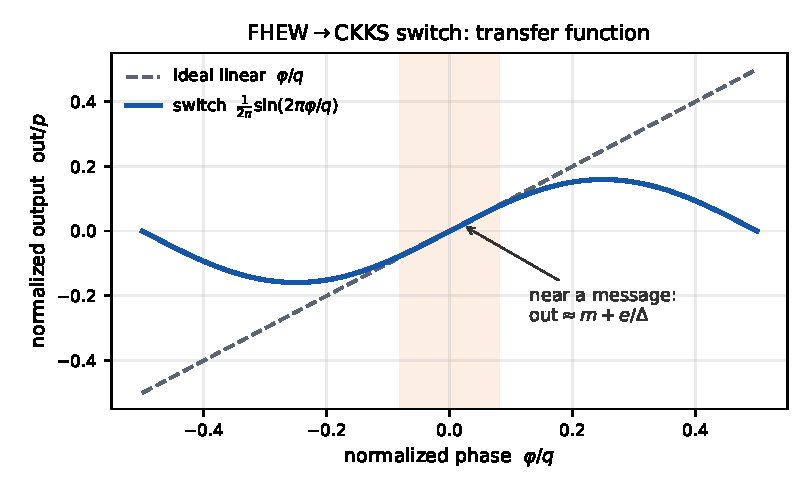
\includegraphics[width=0.62\linewidth]{fig_transfer.pdf}
  \caption{Переключение \fto{} применяет к фазе LWE синусоидальную передаточную функцию вместо округления.
  Вблизи сообщения (заштриховано) выход равен $m + e/\Delta$, так что ошибка LWE
  выживает, ослабленная, внутри пространства сообщений CKKS и восстанавливается обращением синуса.}
  \label{fig:transfer}
\end{figure}

\paragraph{Следствие для контрмеры.}
Утекающая величина $e/\Delta$ --- \emph{доля единицы} сообщения, тот режим, который зашумление
и призвано покрывать. Останавливает ли зашумление эту атаку ---
количественный вопрос, разрешаемый в \S\ref{sec:flooding}.

\section{Атака}
\label{sec:attack}

\paragraph{Модель.}
Мы работаем в игре IND-CPA-D так, как её формулируют~\cite{santato2026} (их Определение~5,
расширенное на конвейеры в Определении~11). Противник управляет тремя оракулами с состоянием.
$E(m_0, m_1)$ шифрует и записывает $(m_0, m_1, ct)$ в состояние. $H(g, J)$ вычисляет допустимую схему
$g$ над имеющимися записями и записывает метки $g(m_0\dots)$, $g(m_1\dots)$. Оракул переключения
$\mathit{SW}$ переносит запись из исходного состояния в целевое, применяя плейнтекст-отображение
$\tau$. Расшифрование --
\[
  D(i):\quad \text{если } S[i].m_0 = S[i].m_1 \ \text{ то вернуть } \mathrm{Dec}(\mathit{sk}, S[i].ct)
  \ \text{ иначе вернуть } \bot
\]
--- заметим, что $D$ берёт \textbf{индекс в состоянии}, а не шифротекст, поданный противником. Это
используется ниже дважды.

\paragraph{Атака.}
Три вызова оракулов:
\begin{enumerate}
  \item $E(0, 0)$ --- свежее FHEW-шифрование нуля входит в состояние с метками $m_0 = m_1 = 0$.
  \item $\mathit{SW}$ --- запись переходит в состояние CKKS с меткой $\tau(0) = 0$.
  \item $D(i)$ --- метки совпадают, поэтому оракул отвечает. Идеальное сообщение --- $0$. Фактическое
    расшифрование --- $e/\Delta$.
\end{enumerate}
Эта разница составляет утечку IND-CPA-D. Из \S\ref{sec:computes} передаточная
функция переключения --- $\out = (p/2\pi)\sin(2\pi\,\varphi/q)$, так что
\[
  e = \frac{q}{2\pi}\,\arcsin\!\left(\out \cdot \frac{2\pi}{p}\right),
\]
восстанавливается точно округлением. Имея ошибку, получаем $\inner{a}{s} = b - e \pmod q$ для
публичных $(a, b)$ --- одно линейное уравнение на шифротекст.

При масштабирующем модуле из собственного примера OpenFHE (50 бит) шум вычислений CKKS забивает
$e/\Delta$, и эта голая форма не срабатывает (единицы точных из $512$ от прогона к прогону). Один
дополнительный вызов оракула это исправляет: применить $H$ с $g(m) = t\cdot m \bmod p$ к записи FHEW
перед переключением. Это плейнтекст-функция --- вызов записывает $g(0) = 0$ --- и она
масштабирует фазу до $t\cdot e$, поднимая сигнал в $t$ раз, тогда как шум CKKS не меняется, поскольку
$a$ масштабируется по модулю $q$ и остаётся равномерным. При $t = 256$ конфигурация по умолчанию уже
даёт $512/512$.

Усиление служит только для измерения: линейное уравнение должно быть записано
с \textbf{исходной} парой $(a, b)$. Использование масштабированной пары и неверно масштабировало бы
ошибку, и для $t$, степени двойки, сделало бы матрицу коэффициентов вырожденной по модулю~$2$, что
разрушает выбор ведущего элемента в решении.

\paragraph{Эффективность.}
Один вызов \code{EvalFHEWtoCKKS} упаковывает до \code{slots} шифротекстов LWE в слоты CKKS, и одно
расшифрование возвращает их все. Один запрос даёт \code{slots} уравнений.

\subsection{Сведение}
Атака формулируется как различитель, чтобы условие выигрыша было явным.

\begin{proposition}
Пусть $\Pi$ --- конвейер \fto{} в OpenFHE при параметрах \S\ref{sec:results}, и пусть \code{slots}
--- число слотов CKKS. Существует противник $\mathcal{A}$, делающий $q = \lceil n/\code{slots}\rceil$
запросов расшифрования (три при наших параметрах) с преимуществом $1/2 - \varepsilon$ в игре
$q$-IND-CPA-D для $\Pi$, где $\varepsilon$ --- вероятность того, что какая-то восстановленная ошибка
неверна либо что никакие $n$ из собранных уравнений не образуют матрицу, обратимую по модулю~$2$.
\end{proposition}

\begin{proof}
$\mathcal{A}$ действует в две фазы.

\emph{Фаза 1 --- извлечение.} Повторять для $j = 1 \dots q$: вызвать $E(0, 0)$ \code{slots} раз,
получив записи состояния с парами меток $(0, 0)$, и записать публичные $(a_i, b_i)$ каждого
возвращённого шифротекста. При необходимости вызвать $H(g_t, \cdot)$ на каждой записи с
$g_t(m) = t\cdot m \bmod p$; вызов записывает $g_t(0) = 0$ с обеих сторон, так что метки по-прежнему
совпадают. Вызвать $\mathit{SW}$ на векторе этих записей; он порождает одну целевую запись с меткой
$\tau(0, \dots, 0) = (0, \dots, 0)$. Вызвать $D$ на этом индексе: две метки совпадают, и оракул
отвечает. Слот $i$ ответа равен
\[
  \out_i = \frac{p}{2\pi}\,\sin\!\left(\frac{2\pi\,t\,e_i}{q}\right) + \eta_i,
\]
где $\eta_i$ --- ошибка вычислений CKKS. $\mathcal{A}$ полагает
$\hat{e}_i = \mathrm{round}\!\big(\tfrac{q}{2\pi t}\arcsin(\out_i \cdot 2\pi/p)\big)$ и записывает
уравнение $\inner{a_i}{s} = b_i - \hat{e}_i \pmod q$ --- записанное с \textbf{исходной} парой
$(a_i, b_i)$, не с масштабированной.

\emph{Фаза 2 --- решение.} $\mathcal{A}$ выбирает $n$ уравнений, чья матрица $A$ обратима по
модулю~$2$, и решает $A x = v \pmod q$ подъёмом Гензеля. Если каждое $\hat{e}_i$ равно $e_i$, то
$x = s$: это утверждение единственности, машинно-проверенное в
\code{lean/LWEKeyRecovery.lean} (\code{secret\_unique}, \code{key\_recovery} и
\code{isUnit\_det\_iff\_map\_two} для выбора по модулю~2). Затем $\mathcal{A}$ вызывает
$E(m_0, m_1)$ с $m_0 \neq m_1$, получая вызов-шифротекст $(a^*, b^*)$; он не может запросить $D$ на
нём, потому что метки различаются --- но ему это и не нужно. $\mathcal{A}$ вычисляет
$m = \mathrm{round}(p\,(b^* - \inner{a^*}{s})/q)$ сам и выводит $0$, если $m = m_0$, иначе $1$.

$\mathcal{A}$ прав, когда извлечение удалось и расшифрование LWE корректно на вызове, так что его
преимущество --- $1/2 - \varepsilon$.
\end{proof}

\paragraph{О $\varepsilon$.}
На $1536$ собранных уравнениях каждая восстановленная
ошибка была точной (\S\ref{sec:results}), а выбранная матрица имела полный ранг $1305$ над
$\mathrm{GF}(2)$. Одна неверная ошибка фатальна: решение тогда возвращает вектор
без единой координаты в $\{-1,0,1\}$. Наши данные дают
оценку по правилу трёх для $\varepsilon$: $0$ отказов на $1536$ даёт поуравненную
точность $\geq 99{.}8\%$ при доверии $95\%$.

\paragraph{Что сведению нужно, а что нет.}
Ему нужны только $E$, $H$ с плейнтекст-функцией, $\mathit{SW}$ и $D$ на индексе, чьи метки совпадают.
Шифротекст собственной сборки на $D$ не подаётся, поэтому сведение допустимо там, где и запрос
ключа переключения из \S\ref{sec:discussion}, и наш собственный ранний пробник
границы недопустимы.

\paragraph{Решение системы.}
Уравнения $\inner{a_j}{s} = v_j \pmod q$ с точными $v_j$ и троичным $s$ решаются напрямую. Поскольку
$q = 2^{28}$ --- степень простого, любые $n$ уравнений, чья матрица обратима по модулю~$2$, имеют
единичный определитель по модулю~$q$; мы выбираем их одним шагом Гаусса над $\mathrm{GF}(2)$ и
поднимаем решение по Гензелю с модуля~$2$ до модуля~$2^{28}$. Алгебраическое ядро этого шага ---
включая утверждение, что решение собранной системы совпадает с секретом, так что противнику не нужен
эталон, чтобы знать, что он попал, --- машинно-проверено в Lean (\code{lean/LWEKeyRecovery.lean}).

\section{Реализация и результаты}
\label{sec:results}

PoC против OpenFHE, коммит \code{ed361af2}.\footnote{Артефакт (proof-of-concept на C\texttt{++},
доказательство в Lean~4 и приводимые здесь логи результатов): \url{\artifacturl}.} CKKS: размерность
кольца $2^{13}$, мультипликативная глубина $13$, перемасштабирование FIXEDAUTO, масштабирующий модуль
$59$ бит. FHEW: STD128, $\log q = 28$, размерность LWE $n = 1305$, $q = 2^{28}$; модуль сообщения LWE
$p = 256$, $\Delta = 2^{20}$. \code{poc/direct.cpp}, $512$ слотов.

\begin{table}[h]
\centering
\begin{tabular}{lr}
\toprule
величина & значение \\
\midrule
уравнений на один запрос расшифрования & $512$ \\
запросов расшифрования на весь ключ ($n = 1305$) & \textbf{3} \\
ошибок восстановлено точно & \textbf{$1536 / 1536$} \\
RMS / макс. ошибка восстановленного $e$ & $0.0104 / 0.0340$ \\
восстановление ключа & \textbf{$1305 / 1305$ координат}, $14{.}8$\,с \\
\bottomrule
\end{tabular}
\end{table}

При настройке из собственного примера OpenFHE (масштабирующий модуль $50$) с шагом усиления
$t = 1024$: $1536/1536$ ошибок точно (RMS $0.016$), и снова \textbf{$1305/1305$ координат}
восстановлены из \textbf{трёх запросов расшифрования}. Взлом покрывает конфигурацию из примера библиотеки.

Решатель также сообщает, что все $1536$ собранных уравнений удовлетворяются восстановленным вектором
--- проверка, не использующая эталон: по теореме единственности противник знает, что ключ у него.

Ранняя версия этой работы локализовала ошибку, проходя сдвигом $b$ по периоду сообщения и
подгоняя получавшийся наклон. Той версии требовалось около $350$ вызовов переключения и
калибровочный пробник, она достигала лишь $0.13$ максимальной ошибки и была
\textbf{недопустима}: сдвиг $b$ на константу, не кратную $\Delta$, не является функцией на
пространстве открытых текстов FHEW, так что $H$ его выполнить не может, а у вызова нет метки для
результата. Прямое считывание заменяет её.

\section{Зашумление: что делает библиотека и что бы потребовалось}
\label{sec:flooding}

\paragraph{(a) Собственная контрмера OpenFHE, реально включённая, атаку не останавливает.}
Установка \code{NOISE\_FLOODING\_DECRYPT} с \code{EXEC\_EVALUATION} и оценкой шума --- это защита,
которую пользователь может включить сегодня. Библиотека ограничивает, насколько её можно выкрутить:
генерация контекста отказывает со словами \emph{<<Precision of less than 3 bits is not supported.
logstd $16.79$ + noiseEstimate $40.0$ must be $56$ or less>>}, так что при этих параметрах оценка не
может превысить $\approx 39.2$. Проходя её вверх до этого потолка:

\begin{table}[h]
\centering
\begin{tabular}{lcccccccc}
\toprule
оценка шума & $10$ & $20$ & $28$ & $32$ & $35$ & $38$ & $39$ & $40$ \\
\midrule
ошибок точно (из $512$) & $512$ & $512$ & $512$ & $512$ & $512$ & $512$ & $\mathbf{512}$ & отказ \\
\bottomrule
\end{tabular}
\end{table}

При любой допустимой настройке, включая наибольшую, которую библиотека соберёт, все $512$ ошибок
по-прежнему восстанавливаются точно (RMS $0.010$--$0.015$). Поставляемая контрмера откалибрована под
ошибку CKKS; считываемая нами величина --- значение в пространстве сообщений размера $e/\Delta$, и
оно выживает.

\paragraph{(b) Синтетическое зашумление фиксированной величины обходится усилением.}
Впрыскивая гауссов шум со стандартным отклонением $\sigma$ прямо в каждый расшифрованный слот, голое
считывание отказывает, как только $\sigma$ превышает около $4$ единиц фазы ($\sigma = 1024$ даёт
$0/40$). Масштабирование шифротекста LWE на $t$ перед переключением его восстанавливает, потому что
сигнал растёт в $t$ раз, а впрыснутый шум --- нет: $0 \to 10 \to 40$ из $40$, когда $t$ идёт
$1 \to 64 \to 1024$.

\paragraph{(c) Зашумление, откалиброванное по распространяемому шумовому тегу, его бы остановило.}
В Алгоритме~6 из~\cite{santato2026} каждый шифротекст несёт шумовой тег, обновляемый при каждой
гомоморфной операции, и расшифрование зашумляет относительно этого тега. Наше усиление --- скалярное
умножение, так что оно умножает и тег. Перезапуская с $\sigma$, масштабируемым пропорционально $t$:

\begin{table}[h]
\centering
\begin{tabular}{lccc}
\toprule
$t$ & $1$ & $64$ & $1024$ \\
\midrule
точно, фиксир. $\sigma$     & $0/40$ & $10/40$ & $40/40$ \\
точно, $\sigma \propto t$ & $0/40$ & $0/40$  & $0/40$ \\
\bottomrule
\end{tabular}
\end{table}

Усиление тогда ничего не даёт, и авторы это прямо предвидят: о собственном усилении $2^k$ они пишут,
что переключение с хорошей гигиеной шифротекстов <<would instead hide from us the new ciphertexts
adaptively on k>>.

\paragraph{Разрыв между (a) и (c).}
Защита, специфицированная в~\cite{santato2026}, работает. Защита, поставляемая в OpenFHE,
слабее, и её нельзя донастроить до нужной силы: библиотека отказывает за
$\approx 39.2$, а величина, масштабированная по тегу и нужная, чтобы покрыть усиленный запрос, много
выше. Нет и запасного пути для противника, когда утечка \emph{покрыта}: остаточная задача, оставляемая
неточным восстановлением ошибки, --- это LWE с $n = 1305$, $q = 2^{28}$ и ошибкой $\sigma \geq 12.6$,
которую штатный Lattice Estimator~\cite{latticeestimator} оценивает в $2^{168}$ и выше ($2^{191}$ и
$2^{216}$ при зашумлённых настройках). Ниже порога точности атака перестаёт работать.

\section{Обсуждение}
\label{sec:discussion}

\paragraph{Возражение про ключ переключения.}
\code{EvalFHEWtoCKKSKeyGen} в OpenFHE задаёт ключ переключения как CKKS-шифрование секрета FHEW ---
комментарий в исходнике говорит ровно это --- и выставляет его через публичный аксессор
\code{cc->GetSwkFC()}. Расшифрование этого ключа возвращает все $1305$ координат сразу; мы это
проверили (\code{poc/swktest.cpp}, макс. ошибка $2\mathrm{e}{-13}$). Отсюда два следствия.

Во-первых, внутри игры этот запрос недопустим: $D$ берёт индекс состояния, а ключ переключения
никогда не является записью состояния, так что противник, ограниченный оракулами, его сделать не
может. Наша атака использует только записи состояния и потому является взломом IND-CPA-D;
тривиальный в этой модели недоступен.

Во-вторых, вне игры тривиальный взлом доминирует. Любое развёртывание, чей сервис расшифрования
принимает произвольный корректный шифротекст CKKS, отдаёт ключ FHEW за один запрос, потому что ключ
переключения является таким шифротекстом. Выставлять не следует ни ключ переключения, ни оракул
расшифрования на переключённых шифротекстах: против последнего достаточно трёх запросов.

\paragraph{Насколько это ново?}
Конвейер, заканчивающийся обычным
расшифрованием CKKS, известен как IND-CPA-D-небезопасный со времён Ли и Миччанчо. Специфично здесь
цель: оракул --- на CKKS, но падает \textbf{FHEW}-секрет. Прямой атаке приходилось усиливать, чтобы перенести ошибку CKKS в пространство
сообщений FHEW; здесь переключение доставляет ошибку LWE в пространство сообщений CKKS без усиления.

\paragraph{Средства защиты.}
Зашумление фиксированной величины недостаточно; зашумление, откалиброванное по распространяемому шумовому тегу,
как в Алгоритме~6 из~\cite{santato2026}, утечку покрывает (\S\ref{sec:flooding}), а гигиена
шифротекстов отказалась бы возвращать компоненту вовсе. OpenFHE не реализует ни
того, ни другого.

\paragraph{Смежные работы и почему они не пересекаются.}
Ближе всего две недавние линии. \citeauthor{liu2025}~\cite{liu2025} атакуют IND-CPA-D-стойкость
\emph{ослабленного функционального бутстрэппинга} в семействе FHEW/TFHE; их рычаг --- вероятность
сбоя бутстрэппинга, а смягчение --- довести эту вероятность до пренебрежимой.
\citeauthor{ogilvie2025}~\cite{ogilvie2025} идёт в другую сторону и строит доказуемую
IND-CPA-D- и KR-D-стойкость для приближённого HE с существенно меньшим шумом расшифрования, чем
прежние доказуемые конструкции, отчасти трактуя шум перемасштабирования как подсказку HintLWE. Эта
работа --- конструктивный аналог нашего \S\ref{sec:flooding}: она показывает, что
малозатратное зашумление с доказуемыми гарантиями существует; поставляемое OpenFHE таким не является. Ни одна из этих работ не касается
изучаемого здесь направления переключения; поиск по
корпусу ePrint по стойкости переключения схем возвращает только~\cite{santato2026}.

\section{Заключение}

Направление \fto{} переключения схем в OpenFHE небезопасно в IND-CPA-D, и дёшево: три запроса
расшифрования восстанавливают полный секретный ключ FHEW STD128, используя только порождённые
оракулами записи состояния. Переключение утекает, потому что выдаёт $m + e/\Delta$ без очистки, так
что ошибка исходной схемы попадает в сообщение целевой. Отдельно, ключ переключения ---
это расшифровываемое шифрование того же секрета, что ломает любое развёртывание, готовое расшифровать
произвольный шифротекст. Защита, предложенная в~\cite{santato2026} --- гигиена шифротекстов с
зашумлением, откалиброванным по распространяемому шумовому тегу, --- по-видимому, закрывает первую
брешь, и наши измерения это подтверждают; вторая закрывается тем, чтобы не публиковать ключ. Ни то,
ни другое не реализовано в том, что пользователи получают сегодня.

\bibliographystyle{plainnat}
\bibliography{refs}

\end{document}
